\section{Результаты измерений}

\subsection{Определение по измерениям растяжения проволоки}

По информации со стенда
\[d=0{,}73\,\text{мм}\]
\[S=\frac{\pi d^2}{4}=0{,}42\,\text{мм}^2\]

Длина проволоки
\[l=175{,}7\pm 0{,}05\text{см}\]

Изменение числа делений связано с увеличением длины проволоки связано соотношением
\[\Delta l = \frac{nr}{2h}\]
$r=13\,\text{см}$~--- длина рычага, $h=137{,}8\,\text{см}$~--- расстояние от зеркала
до шкалы.

\begin{table}[!ht]
    \centering
    \caption{Зависимость растяжения от массы добавленного груза}
    \begin{tabular}{|l|l|l|l|l|l|}
    \hline
        $n_1,\,\pm 0{,}5\text{мм}$ & $m_1,\,\pm 0{,}05\text{г}$ & $n_2,\,\pm 0{,}5\text{мм}$ & $m_2,\,\pm 0{,}05\text{г}$ & $n_3,\,\pm 0{,}5\text{мм}$ & $m_3,\,\pm 0{,}05\text{г}$ \\ \hline
        128 & 0 & ~ & 0 & 121 & 0 \\ \hline
        138 & 246.1 & 141 & 246.1 & 132 & 245.5 \\ \hline
        148 & 245.7 & 153 & 245.6 & 144 & 245.6 \\ \hline
        159 & 246.1 & 165 & 245.5 & 156 & 246.1 \\ \hline
        179 & 245.8 & 176 & 245.8 & 169 & 245.5 \\ \hline
        182 & 245.6 & 189 & 247.7 & 179 & 245.7 \\ \hline
        193 & 245.5 & 199 & 245.5 & 190 & 245.8 \\ \hline
        205 & 245.5 & 210 & 245.6 & 221 & 245.7 \\ \hline
        216 & 245.6 & 223 & 246.1 & 212 & 246.1 \\ \hline
        224 & 245.7 & 235 & 245.7 & ~ & ~ \\ \hline
    \end{tabular}
\end{table}

Общая масса грузов на измерении в строке $i$ равна сумме масс грузов, записанных
выше этой строки. 

На основе данных в таблице посчитаем $\Delta l$ и построим график удлинения проволоки
от силы, действующей на неё.

\begin{figure}[h!]
    \center{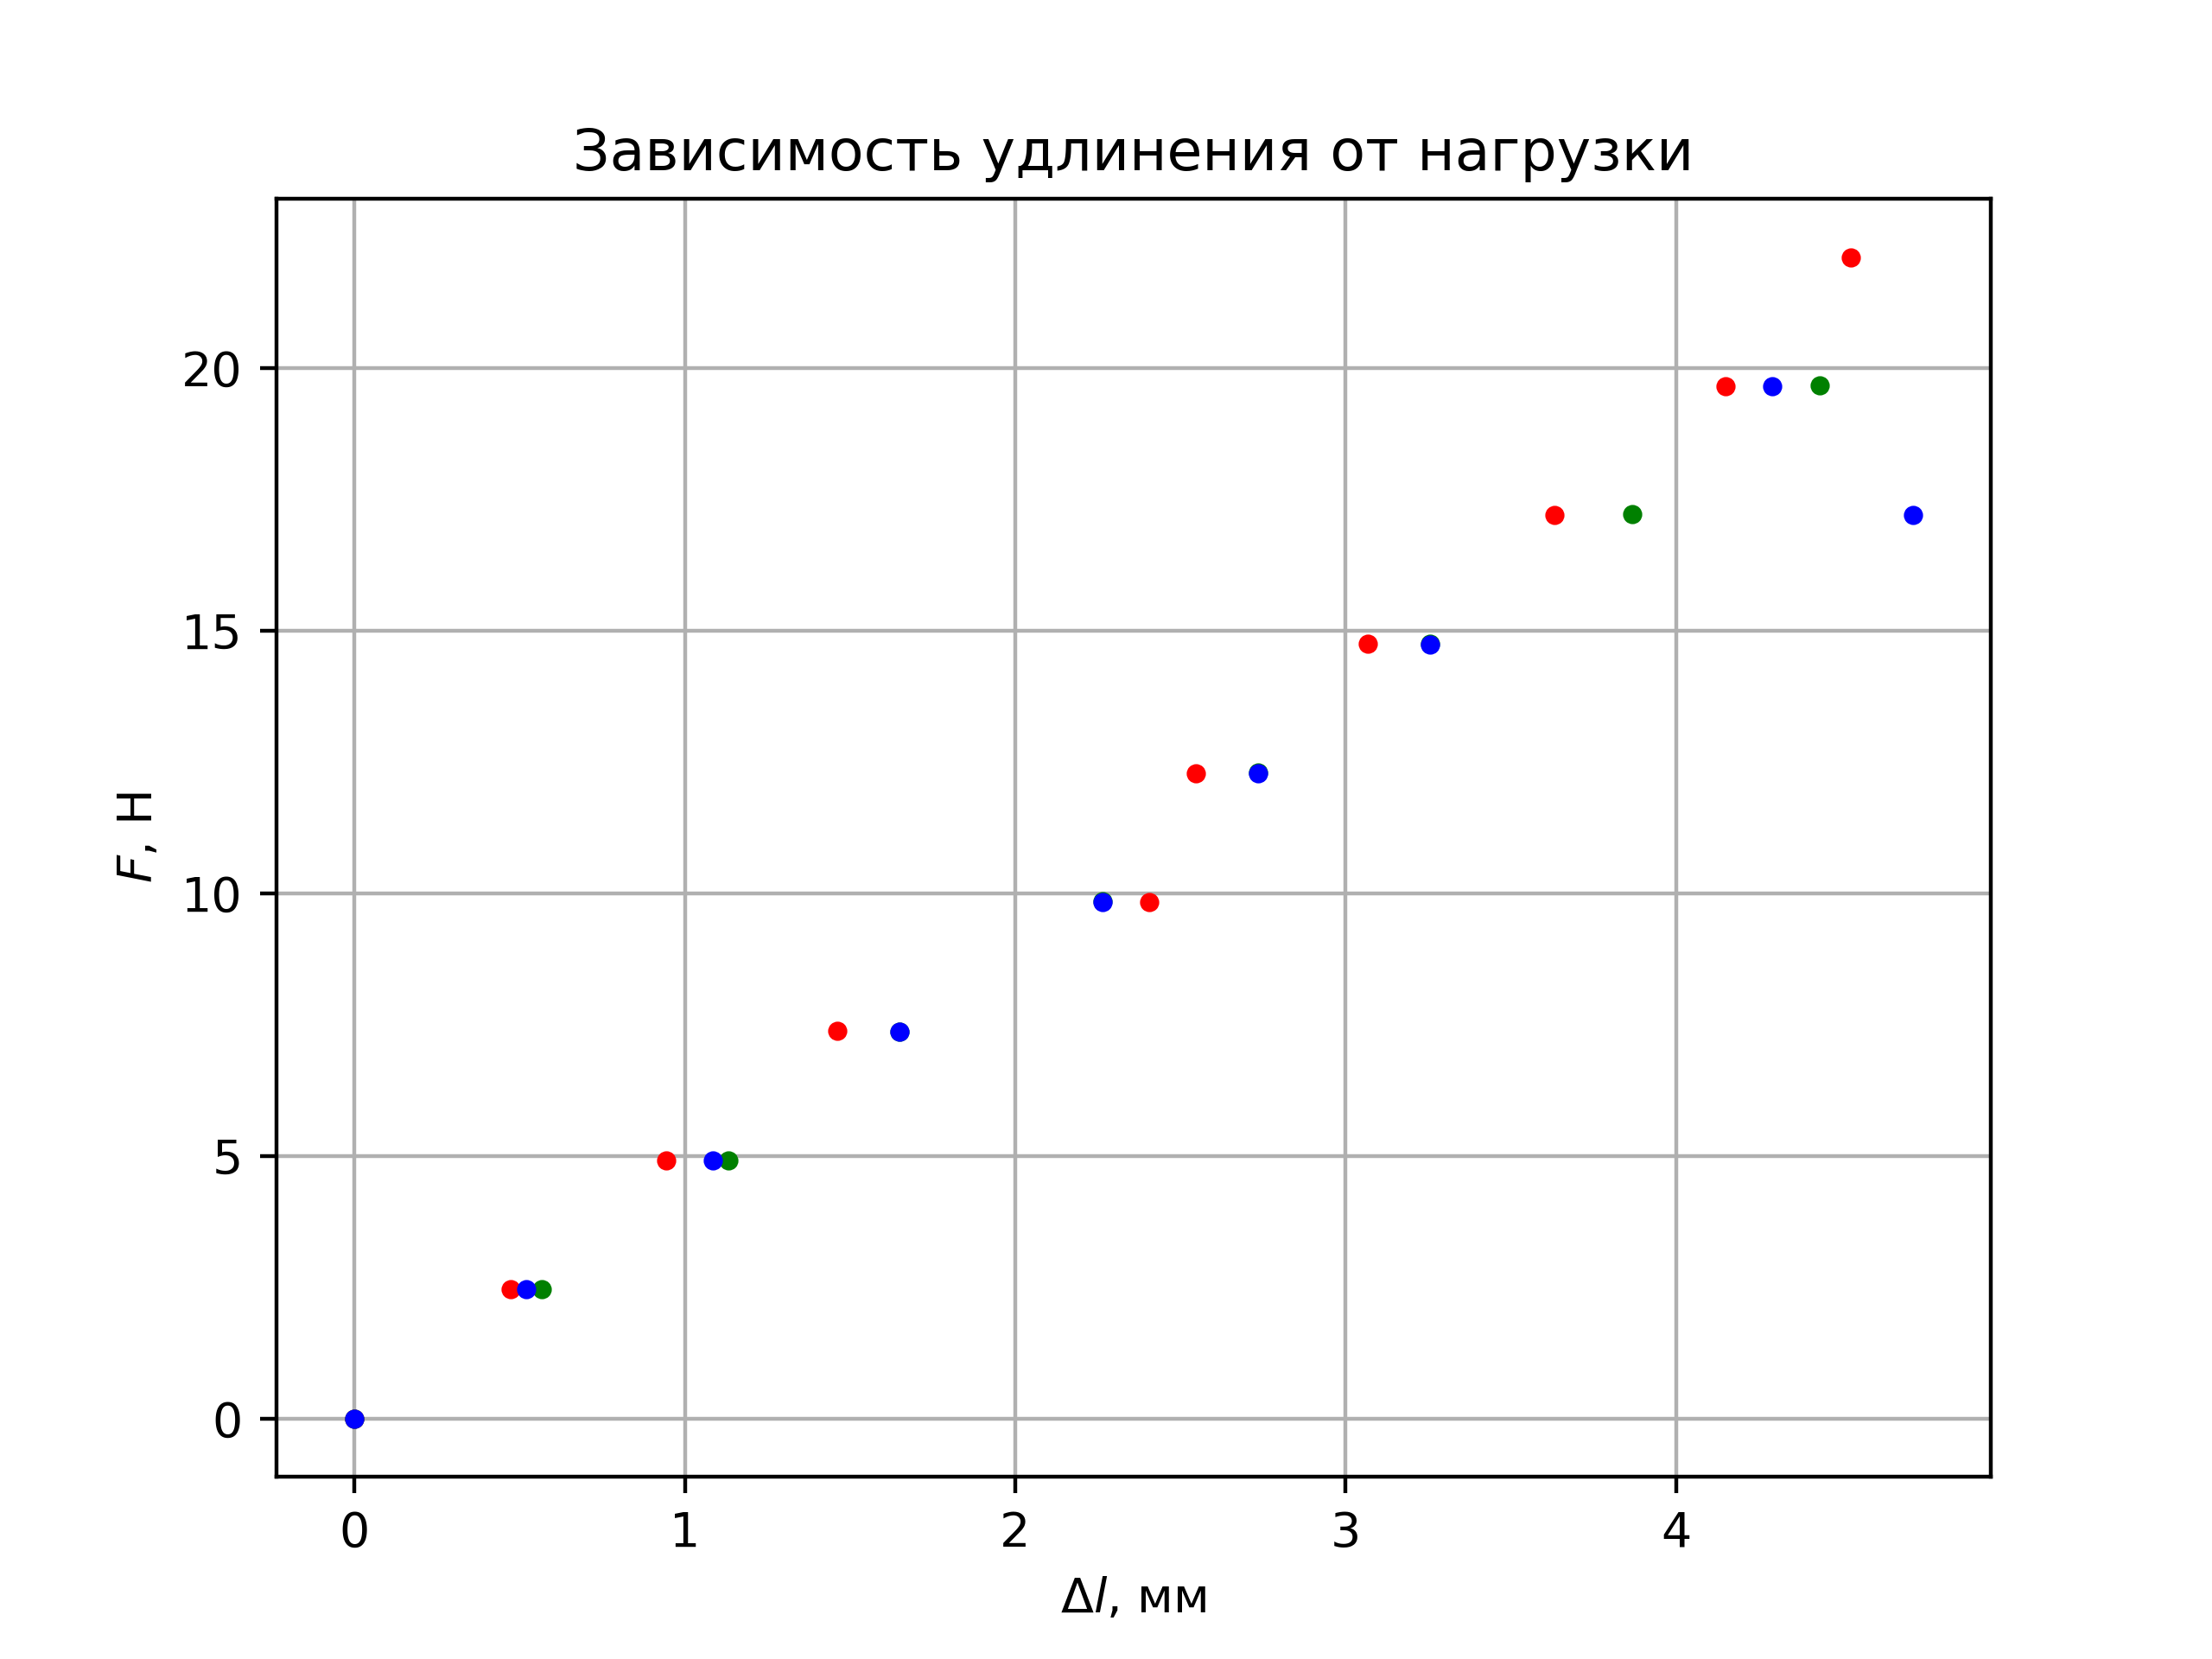
\includegraphics[width=0.8\linewidth]{img/dirty.png}}
\end{figure}

Уберём выбросную точку при $n_3=221\,\text{мм}$ и по МНК проведём усредняющую прямую.
\begin{figure}[h!]
    \center{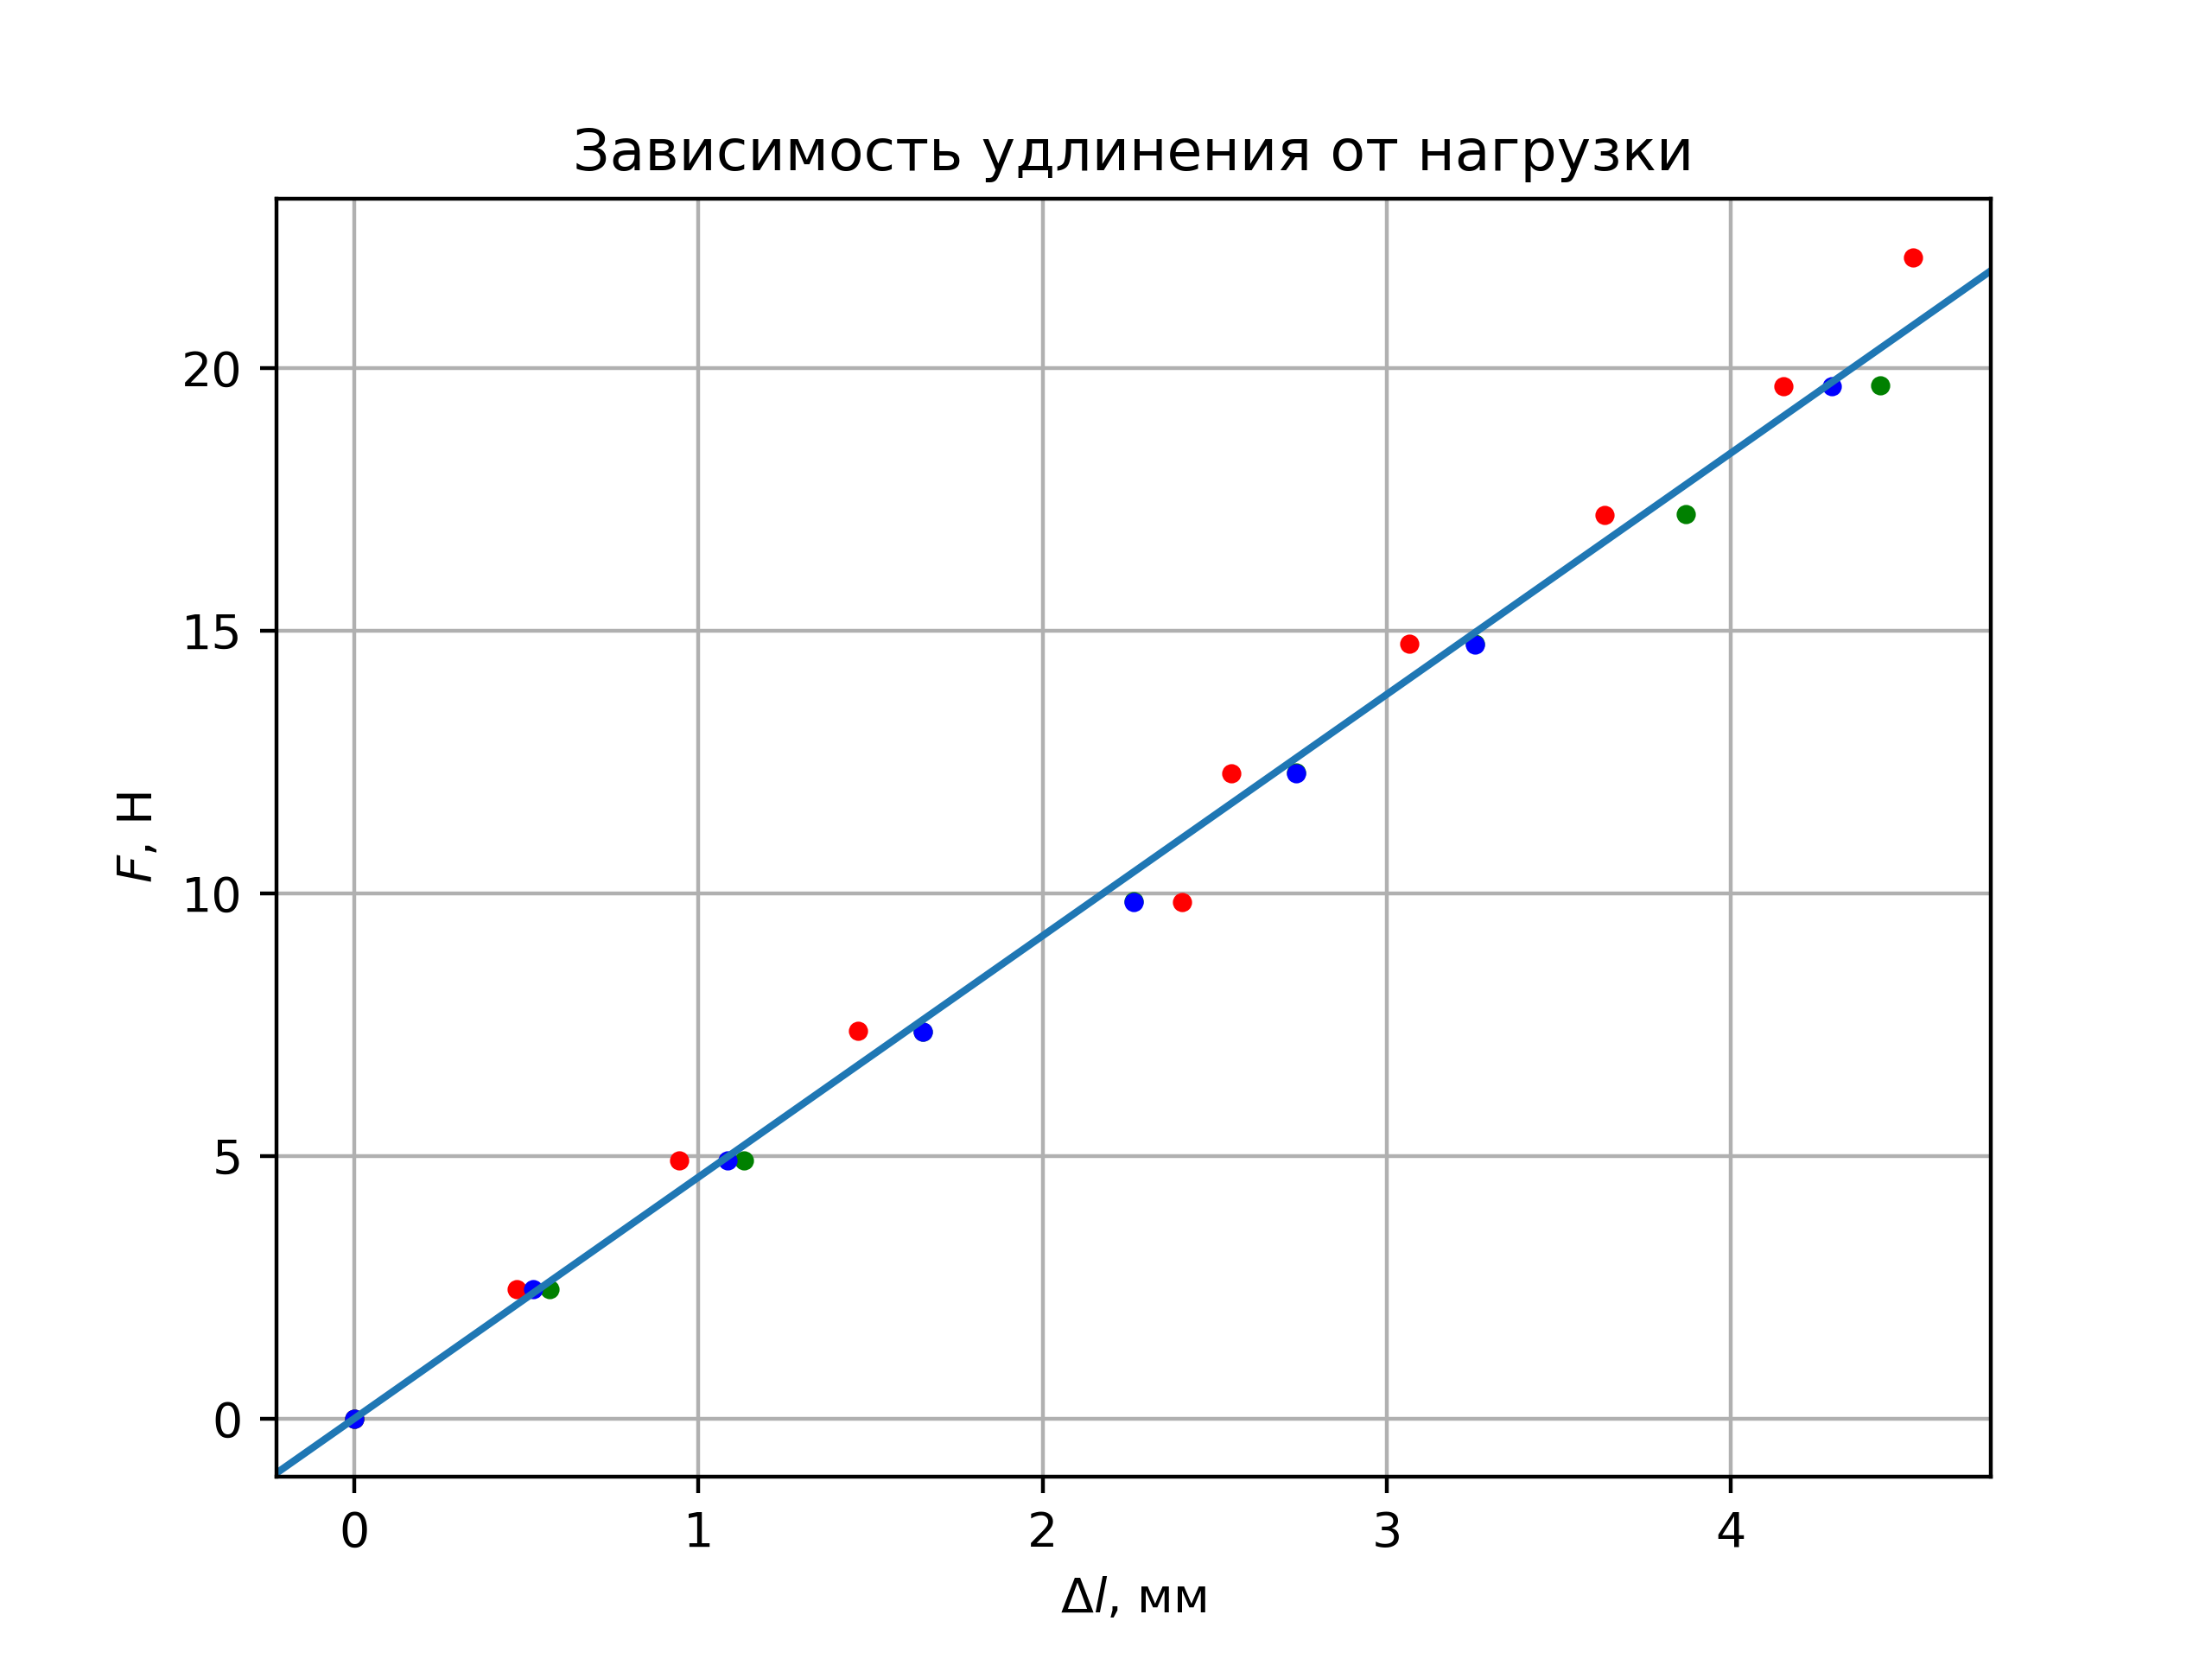
\includegraphics[width=0.8\linewidth]{img/clean.png}}
\end{figure}

Получаем $k=4600\pm 50\,\text{Н}/\text{м}$ ($\varepsilon\approx 0{,}01$).
Относительные погрешности измерений $m$ и $l$ на несколько порядков меньше $0{,}01$,
а влияние погрешности измерений $n$ мало, т.к. $\varepsilon_n\approx \frac{\delta n}{\Delta n}\approx 0{,}005$.

\[E=k\frac{l}{S}=\left(1{,}93\pm 0{,}02\right)\cdot 10^{11 }\,\text{Па}\]

Такое значение модуля Юнга соответствует стали.

\subsection{Определение модуля Юнга по изгибу балки}

Расстояние между рёбрами призмам
\[l_{AB}=51\pm 0{,}05\,\text{см}\]

Измерим толщину $b$ и ширину $a$ всех четырёх балок.

\begin{table}[!ht]
    \centering
    \caption{Измерение длин и толщин балок}
    \begin{tabular}{|l|l|l|l|l|l|l|l|l|l|l|}
    \hline
    $a_1\,\pm 0{,}05\text{мм}$ & 20.0 & 19.8 & 19.4 & 19.6 & 19.7 & 19.7 & 19.9 & 19.7 & 19.8 & 20.2 \\ \hline
    $b_1\,\pm 0{,}05\text{мм}$ & 9.3 & 9.4 & 9.4 & 9.2 & 9.3 & 9.3 & 9.2 & 9.3 & 9.3 & 9.3 \\ \hline
    $a_2\,\pm 0{,}05\text{мм}$ & 21.8 & 21.6 & 21.5 & 21.5 & 21.2 & 21.5 & 21.2 & 21.4 & 21.4 & 22.0 \\ \hline
    $b_2\,\pm 0{,}05\text{мм}$ & 10.9 & 10.9 & 11.1 & 11.0 & 10.9 & 10.7 & 10.9 & 11.2 & 11.4 & 11.1 \\ \hline
    $a_3\,\pm 0{,}05\text{мм}$ & 21.5 & 21.3 & 21.3 & 21.4 & 21.5 & 21.5 & 21.5 & 21.6 & 21.5 & 21.5 \\ \hline
    $b_3\,\pm 0{,}05\text{мм}$ & 4.3 & 4.2 & 4.1 & 4.1 & 4.0 & 3.9 & 3.9 & 4.0 & 3.9 & 4.0 \\ \hline
    $a_4\,\pm 0{,}05\text{мм}$ & 21.2 & 21.4 & 21.2 & 21.1 & 21.1 & 21.0 & 21.0 & 21.0 & 21.0 & 21.4 \\ \hline
    $b_4\,\pm 0{,}05\text{мм}$ & 4.0 & 4.0 & 3.9 & 3.9 & 3.9 & 3.8 & 3.9 & 3.9 & 3.9 & 4.0 \\ \hline
    \end{tabular}
\end{table}
\newpage
~
\newpage
Итого
\begin{gather*}
    a_1 = 19{,}78\pm 0{,}16\,\text{мм}\;\;\text{(}\varepsilon = 0{,}8\%\text{)}\\
    b_1 = 9{,}3\pm 0{,}1\,\text{мм}\;\;\text{(}\varepsilon = 1\%\text{)} \\
    a_2 = 21{,}51\pm 0{,}16\,\text{мм}\;\;\text{(}\varepsilon = 0{,}7\%\text{)} \\
    b_2 = 11{,}01\pm 0{,}15\,\text{мм}\;\;\text{(}\varepsilon = 1{,}4\%\text{)} \\
    a_3 = 21{,}46\pm 0{,}11\,\text{мм}\;\;\text{(}\varepsilon = 0{,}5\%\text{)} \\
    b_3 = 4{,}04\pm 0{,}13\,\text{мм}\;\;\text{(}\varepsilon = 3{,}2\%\text{)} \\
    a_4 = 21{,}14\pm 0{,}14\,\text{мм}\;\;\text{(}\varepsilon = 0{,}6\%\text{)} \\
    b_4 = 3{,}92\pm 0{,}09\,\text{мм}\;\;\text{(}\varepsilon = 2{,}3\%\text{)}
\end{gather*}

\begin{table}[!ht]
    \centering
    \caption{Изменение прогиба балок}
    \begin{tabular}{|l|l|l|l|l|l|l|l|l|}
    \hline
        $m,\text{г}$ & $y_{11}$ & $y_{12}$ & $y_{21}$ & $y_{22}$ & $y_{31}$ & $y_{32}$ & $y_{41}$ & $y_{42}$ \\ \hline
        0 & 667 & 628 & 781 & 731 & 988 & 935 & 819 & 703 \\ \hline
        504 & 601 & 570 & 705 & 659 & 862 & 813 & 750 & 632 \\ \hline
        1001.3 & 537 & 507 & 634 & 589 & 740 & 689 & 681 & 562 \\ \hline
        1457.9 & 476 & 448 & 568 & 522 & 628 & 578 & 618 & 498 \\ \hline
        1925.5 & 415 & 386 & 498 & 463 & 512 & 460 & 554 & 432 \\ \hline
        2380.3 & 354 & 326 & 432 & 393 & 400 & 349 & 490 & 367 \\ \hline
        2884.7 & 288 & 276 & 358 & 318 & 278 & 223 & 421 & 296 \\ \hline
        3358.6 & 226 & 219 & 288 & 247 & 160 & 105 & 355 & 228 \\ \hline
        3860 & 159 & 153 & 215 & 170 & 37 & ~ & 285 & 156 \\ \hline
        3358.6 & 223 & 210 & 282 & 239 & 160 & 105 & 352 & 225 \\ \hline
        2884.7 & 285 & 268 & 348 & 306 & 273 & 220 & 417 & 291 \\ \hline
        2380.3 & 350 & 319 & 420 & 379 & 397 & 347 & 487 & 360 \\ \hline
        1925.5 & 410 & 378 & 485 & 442 & 509 & 458 & 549 & 424 \\ \hline
        1457.9 & 472 & 439 & 552 & 508 & 624 & 574 & 614 & 489 \\ \hline
        1001.3 & 533 & 497 & 618 & 574 & 739 & 686 & 678 & 552 \\ \hline
        504 & 598 & 560 & 692 & 642 & 861 & 810 & 745 & 621 \\ \hline
        0 & 665 & 623 & 770 & 715 & 987 & 934 & 816 & 692 \\ \hline
    \end{tabular}
\end{table}
Первая цифра в $y_{**}$~--- номер балки, а вторая~--- положение ($1$~--- одной стороной и
$2$~--- другой). Значения $y_{**}$ даны в десятках микрометров с погрешностью $5\,\text{мкм}$.
Пропущенное значение $y_{32}$ возникло из-за зашкала прибора.

При небольших смещениях ($\sim 4\,\text{мм}$) от центра показания при максимальной
массе грузов изменяются примерно на $0{,}2\,\text{мм}$. Вторая (деревянная) и третья
(из металла) балки прогибаются несимметрично.

Все балки возвращаются в исходное положение после снятия грузов (с точностью до
$0{,}1\,\text{мм}$).

При переворачивании балки 1 и 2 (деревянные) сильно меняют свой модуль Юнга,
а 3 и 4 (металлические) почти не меняют их.

\newcommand{\graph}[1]{\begin{figure}[h!]\center{\includegraphics[width=0.8\linewidth]{img/#1.png}}\end{figure}}

\graph{dy11}
\graph{dy12}
\newpage ~
\graph{dy21}
\graph{dy22}
\newpage ~
\graph{dy31}
\graph{dy32}
\newpage ~
\graph{dy41}
\graph{dy42}
\newpage ~

\begin{gather*}
    k_{11} = 7580\pm 460\,\text{Н}/\text{м}\;\;\text{(}\varepsilon = 6\%\text{)} \\
    k_{12} = 8020\pm 490\,\text{Н}/\text{м}\;\;\text{(}\varepsilon = 6\%\text{)} \\
    k_{21} = 6730\pm 420\,\text{Н}/\text{м}\;\;\text{(}\varepsilon = 6\%\text{)} \\
    k_{22} = 6870\pm 430\,\text{Н}/\text{м}\;\;\text{(}\varepsilon = 6\%\text{)} \\
    k_{31} = 4050\pm 250\,\text{Н}/\text{м}\;\;\text{(}\varepsilon = 6\%\text{)} \\
    k_{32} = 4050\pm 260\,\text{Н}/\text{м}\;\;\text{(}\varepsilon = 6\%\text{)} \\
    k_{41} = 7210\pm 440\,\text{Н}/\text{м}\;\;\text{(}\varepsilon = 6\%\text{)} \\
    k_{42} = 7020\pm 430\,\text{Н}/\text{м}\;\;\text{(}\varepsilon = 6\%\text{)}
\end{gather*}

Погрешностью измерения $\Delta y$ можно пренебречь, т.к. она очень мала ($\sim 0{,}005$).

\[E = k\frac{l^3}{4ab^3}\]

\begin{gather*}
    E_{11} = \left(1{,}58\pm 0{,}12\right)\cdot 10^{10}\,\text{Па} \\
    E_{12} = \left(1{,}67\pm 0{,}13\right)\cdot 10^{10}\,\text{Па} \\
    E_{21} = \left(7{,}77\pm 0{,}62\right)\cdot 10^{9}\,\text{Па} \\
    E_{22} = \left(7{,}93\pm 0{,}63\right)\cdot 10^{9}\,\text{Па} \\
    E_{31} = \left(9{,}49\pm 1{,}07\right)\cdot 10^{10}\,\text{Па} \\
    E_{32} = \left(9{,}49\pm 1{,}09\right)\cdot 10^{10}\,\text{Па} \\
    E_{41} = \left(1{,}88\pm 0{,}18\right)\cdot 10^{11}\,\text{Па} \\
    E_{42} = \left(1{,}82\pm 0{,}17\right)\cdot 10^{11}\,\text{Па}
\end{gather*}

Усредним значения
\begin{gather*}
    E_{1} = \left(1{,}63\pm 0{,}13\right)\cdot 10^{10}\,\text{Па} \\
    E_{2} = \left(7{,}85\pm 0{,}63\right)\cdot 10^{9}\,\text{Па} \\
    E_{3} = \left(9{,}49\pm 1{,}09\right)\cdot 10^{10}\,\text{Па} \\
    E_{4} = \left(1{,}85\pm 0{,}18\right)\cdot 10^{11}\,\text{Па}
\end{gather*}

Балка 4 сделана из железа, третья~--- из латуни, остальные~--- деревянные.
